\documentclass{standalone}
\usepackage{tikz}
\usepackage{hyperref}
\usepackage{dictsym}

\usetikzlibrary{shadows,calc,math,shadings}


\newcommand{\html}[2]{\href{../html/#1/explanations.html}{#2}}
% \newcommand{\mathy}{\dsmathematical}
\newcommand{\mathy}{}



% TODO: samplers using callbacks

\begin{document}

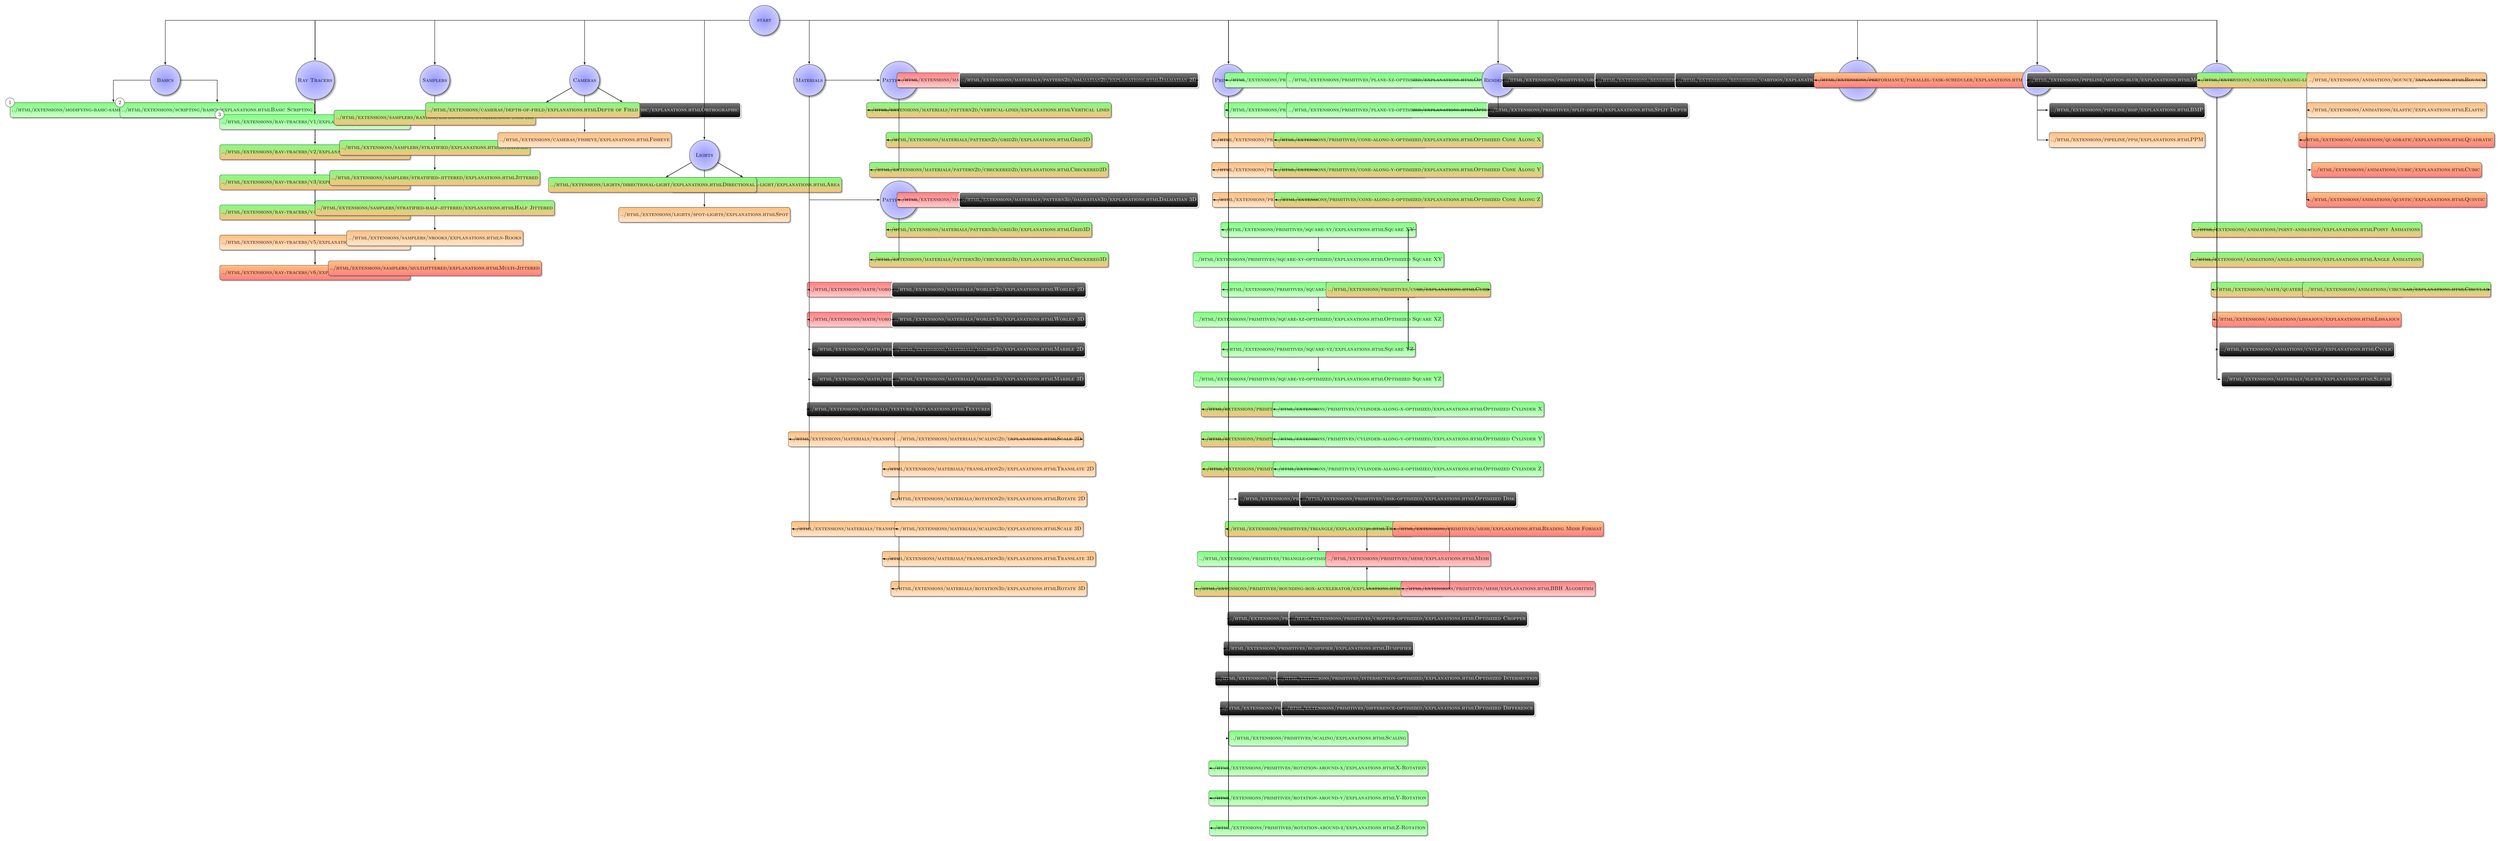
\begin{tikzpicture}[extension/.style={draw,minimum width=5cm,minimum height=1cm,font=\scshape,rounded corners=4pt,drop shadow},
                    dependency/.style={thick,latex-},
                    node/.style={circle,draw,shading=radial,minimum size=2cm,inner color=blue!40,outer color=blue!20,font=\scshape,circular drop shadow},
                    area/.style={left color=gray!30,right color=gray!10,rounded corners=4pt},
                    easy/.style={top color=green!50,bottom color=green!20},
                    medium/.style={top color=orange!50,bottom color=orange!20},
                    hard/.style={top color=red!50,bottom color=red!20},
                    order/.style={draw,circle,fill=white},
                    difficulty1/.style={easy},
                    difficulty2/.style={top color=green!50,bottom color=orange!50},
                    difficulty3/.style={medium},
                    difficulty4/.style={top color=orange!50,bottom color=red!50},
                    difficulty5/.style={hard},
                    difficulty/.style={difficulty#1},
                    todo/.style={white,top color=gray,bottom color=black,ultra thick}]
  \pgfdeclarelayer{background}
  \pgfdeclarelayer{foreground}
  \pgfsetlayers{background,main,foreground}

  \begin{pgfonlayer}{main}
    \node[node] (start) {start};

    \node[node] (basics) at ($ (start) + (-40, -4) $) {Basics};
    \draw[dependency] (basics) |- (start);

    \node[extension,difficulty=1] (modifying basic sample) at ($ (basics) + (-150:4) $) {\html{extensions/modifying-basic-sample}{Basic Sample}};
    \draw[dependency] (modifying basic sample) |- (basics);

    \node[extension,easy] (scripting basics) at ($ (basics) + (-30:4) $) {\html{extensions/scripting/basics}{Basic Scripting}};
    \draw[dependency] (scripting basics) |- (basics);

    \node[node] (ray tracers) at ($ (basics) + (10,0) $) {Ray Tracers};
    \draw[dependency] (ray tracers) |- (start);

    \node[extension,anchor=north,easy] (ray tracer v1) at ($ (ray tracers.south) + (0,-1) $) {\html{extensions/ray-tracers/v1}{Ray Tracer v1}};
    \draw[dependency] (ray tracer v1) -- (ray tracers);

    \node[extension,anchor=north,difficulty=2] (ray tracer v2) at ($ (ray tracer v1.south) + (0,-1) $) {\html{extensions/ray-tracers/v2}{Ray Tracer v2}};
    \draw[dependency] (ray tracer v2) -- (ray tracer v1);

    \node[extension,anchor=north,difficulty=2] (ray tracer v3) at ($ (ray tracer v2.south) + (0,-1) $) {\html{extensions/ray-tracers/v3}{Ray Tracer v3}};
    \draw[dependency] (ray tracer v3) -- (ray tracer v2);

    \node[extension,anchor=north,difficulty=2] (ray tracer v4) at ($ (ray tracer v3.south) + (0,-1) $) {\html{extensions/ray-tracers/v4}{Ray Tracer v4}};
    \draw[dependency] (ray tracer v4) -- (ray tracer v3);

    \node[extension,anchor=north,difficulty=3] (ray tracer v5) at ($ (ray tracer v4.south) + (0,-1) $) {\html{extensions/ray-tracers/v5}{Ray Tracer v5}};
    \draw[dependency] (ray tracer v5) -- (ray tracer v4);

    \node[extension,anchor=north,difficulty=4] (ray tracer v6) at ($ (ray tracer v5.south) + (0,-1) $) {\html{extensions/ray-tracers/v6}{Ray Tracer v6}};
    \draw[dependency] (ray tracer v6) -- (ray tracer v5);

    \node[node] (samplers) at ($ (ray tracers) + (8,0) $) {Samplers};
    \draw[dependency] (samplers) |- (start);

    \node[extension,anchor=north,difficulty=2] (random sampler) at ($ (samplers) + (0,-2) $) {\html{extensions/samplers/random}{Random Sampler}};
    \draw[dependency] (random sampler) -- (samplers);

    \node[extension,anchor=north,difficulty=2] (stratified sampler) at ($ (random sampler.south) + (0,-1) $) {\html{extensions/samplers/stratified}{Stratified}};
    \draw[dependency] (stratified sampler) -- (random sampler);

    \node[extension,anchor=north,difficulty=2] (jittered sampler) at ($ (stratified sampler.south) + (0,-1) $) {\html{extensions/samplers/stratified-jittered}{Jittered}};
    \draw[dependency] (jittered sampler) -- (stratified sampler);

    \node[extension,anchor=north,difficulty=2] (half jittered sampler) at ($ (jittered sampler.south) + (0,-1) $) {\html{extensions/samplers/stratified-half-jittered}{Half Jittered}};
    \draw[dependency] (half jittered sampler) -- (jittered sampler);

    \node[extension,anchor=north,difficulty=3] (nrooks sampler) at ($ (half jittered sampler.south) + (0,-1) $) {\html{extensions/samplers/nrooks}{n-Rooks}};
    \draw[dependency] (nrooks sampler) -- (half jittered sampler);

    \node[extension,anchor=north,difficulty=4] (multijittered sampler) at ($ (nrooks sampler.south) + (0,-1) $) {\html{extensions/samplers/multijittered}{Multi-Jittered}};
    \draw[dependency] (multijittered sampler) -- (nrooks sampler);

    \node[node] (cameras) at ($ (samplers) + (10,0) $) {Cameras};
    \draw[dependency] (cameras) |- (start);

    \node[extension,medium,todo] (orthographic camera) at ($ (cameras) + (-30:4) $) {\html{extensions/cameras/orthographic}{Orthographic}};
    \draw[dependency] (orthographic camera) -- (cameras);

    \node[extension,medium] (fisheye camera) at ($ (cameras) + (-90:4) $) {\html{extensions/cameras/fisheye}{Fisheye}};
    \draw[dependency] (fisheye camera) -- (cameras);

    \node[extension,difficulty=2] (depth of field camera) at ($ (cameras) + (-150:4) $) {\html{extensions/cameras/depth-of-field}{Depth of Field}};
    \draw[dependency] (depth of field camera) -- (cameras);

    \node[node] (lights) at ($ (cameras) + (8,-5) $) {Lights};
    \draw[dependency] (lights) |- (start);

    \node[extension,difficulty=2] (area light) at ($ (lights) + (-30:4) $) {\html{extensions/lights/area-light}{Area}};
    \draw[dependency] (area light) -- (lights);

    \node[extension,difficulty=3] (spot light) at ($ (lights) + (-90:4) $) {\html{extensions/lights/spot-lights}{Spot}};
    \draw[dependency] (spot light) -- (lights);

    \node[extension,difficulty=2] (directional light) at ($ (lights) + (-150:4) $) {\html{extensions/lights/directional-light}{Directional}};
    \draw[dependency] (directional light) -- (lights);

    \node[node] (materials) at ($ (cameras) + (15,0) $) {Materials};
    \draw[dependency] (materials) |- (start);

    \node[node] (pattern 2d materials) at ($ (materials) + (6,0) $) {Patterns 2D};
    \draw[dependency] (pattern 2d materials) -- (materials);

    \node[extension,difficulty=5] (voronoi 2d 1) at ($ (pattern 2d materials) + (6,0) $) {\html{extensions/math/voronoi2d}{Voronoi 2D} \mathy};
    \draw[dependency] (voronoi 2d 1) -- (pattern 2d materials);

    \node[extension,hard,todo] (dalmatian 2d material) at ($ (voronoi 2d 1) + (6,0) $) {\html{extensions/materials/pattern2d/dalmatian2d}{Dalmatian 2D}};
    \draw[dependency] (dalmatian 2d material) -- (voronoi 2d 1);

    \node[node] (pattern 3d materials) at ($ (materials) + (6,-8) $) {Patterns 3D};
    \draw[dependency] (pattern 3d materials) -| (materials);

    \node[extension,difficulty=5] (voronoi 3d 1) at ($ (pattern 3d materials) + (6,0) $) {\html{extensions/math/voronoi3d}{Voronoi 3D} \mathy};
    \draw[dependency] (voronoi 3d 1) -- (pattern 3d materials);

    \node[extension,difficulty=2] (grid3d pattern material) at ($ (voronoi 3d 1) + (0,-2) $) {\html{extensions/materials/pattern3d/grid3d}{Grid3D}};
    \draw[dependency] (grid3d pattern material) -| (pattern 3d materials);

    \node[extension,difficulty=2] (checkered3d pattern material) at ($ (grid3d pattern material) + (0,-2) $) {\html{extensions/materials/pattern3d/checkered3d}{Checkered3D}};
    \draw[dependency] (checkered3d pattern material) -| (pattern 3d materials);

    \node[extension,hard,todo] (dalmatian 3d material) at ($ (voronoi 3d 1) + (6,0) $) {\html{extensions/materials/pattern3d/dalmatian3d}{Dalmatian 3D}};
    \draw[dependency] (dalmatian 3d material) -| (voronoi 3d 1);

    \node[extension,difficulty=5] (voronoi 2d 2) at ($ (materials) + (6,-14) $) {\html{extensions/math/voronoi2d}{Voronoi 2D} \mathy};
    \draw[dependency] (voronoi 2d 2) -| (materials);

    \node[extension,medium,todo] (worley 2d material) at ($ (voronoi 2d 2) + (6,0) $) {\html{extensions/materials/worley2d}{Worley 2D}};
    \draw[dependency] (worley 2d material) -| (voronoi 2d 2);

    \node[extension,difficulty=5] (voronoi 3d 2) at ($ (voronoi 2d 2) + (0,-2) $) {\html{extensions/math/voronoi3d}{Voronoi 3D} \mathy};
    \draw[dependency] (voronoi 3d 2) -| (materials);

    \node[extension,medium,todo] (worley 3d material) at ($ (voronoi 3d 2) + (6,0) $) {\html{extensions/materials/worley3d}{Worley 3D}};
    \draw[dependency] (worley 3d material) -| (voronoi 3d 2);

    \node[extension,difficulty=2] (vertical lines pattern material) at ($ (voronoi 2d 1) + (0,-2) $) {\html{extensions/materials/pattern2d/vertical-lines}{Vertical lines}};
    \draw[dependency] (vertical lines pattern material) -| (pattern 2d materials);

    \node[extension,difficulty=2] (grid2d pattern material) at ($ (vertical lines pattern material) + (0,-2) $) {\html{extensions/materials/pattern2d/grid2d}{Grid2D}};
    \draw[dependency] (grid2d pattern material) -| (pattern 2d materials);

    \node[extension,difficulty=2] (checkered 2d pattern material) at ($ (grid2d pattern material) + (0,-2) $) {\html{extensions/materials/pattern2d/checkered2d}{Checkered2D}};
    \draw[dependency] (checkered 2d pattern material) -| (pattern 2d materials);

    \node[extension,hard,todo] (perlin 2d) at ($ (voronoi 3d 2) + (0,-2) $) {\html{extensions/math/perlin2d}{Perlin 2D} \mathy};
    \draw[dependency] (perlin 2d) -| (materials);

    \node[extension,medium,todo] (marble 2d material) at ($ (perlin 2d) + (6,0) $) {\html{extensions/materials/marble2d}{Marble 2D}};
    \draw[dependency] (marble 2d material) -- (perlin 2d);

    \node[extension,hard,todo] (perlin 3d) at ($ (perlin 2d) + (0,-2) $) {\html{extensions/math/perlin3d}{Perlin 3D} \mathy};
    \draw[dependency] (perlin 3d) -| (materials);

    \node[extension,medium,todo] (marble 3d material) at ($ (perlin 3d) + (6,0) $) {\html{extensions/materials/marble3d}{Marble 3D}};
    \draw[dependency] (marble 3d material) -| (perlin 3d);

    \node[extension,medium,todo] (texture materials) at ($ (perlin 3d) + (0,-2) $) {\html{extensions/materials/texture}{Textures}};
    \draw[dependency] (texture materials) -| (materials);

    \node[extension,difficulty=3] (material transformer 2d) at ($ (texture materials) + (0,-2) $) {\html{extensions/materials/transformer2d}{Transformer2D}};
    \draw[dependency] (material transformer 2d) -| (materials);

    \node[extension,difficulty=3] (material scale 2d) at ($ (material transformer 2d) + (6,0) $) {\html{extensions/materials/scaling2d}{Scale 2D}};
    \draw[dependency] (material scale 2d) -- (material transformer 2d);

    \node[extension,difficulty=3] (material translate 2d) at ($ (material scale 2d) + (0,-2) $) {\html{extensions/materials/translation2d}{Translate 2D}};
    \draw[dependency] (material translate 2d) -| (material transformer 2d);

    \node[extension,difficulty=3] (material rotate 2d) at ($ (material translate 2d) + (0,-2) $) {\html{extensions/materials/rotation2d}{Rotate 2D}};
    \draw[dependency] (material rotate 2d) -| (material transformer 2d);

    \node[extension,difficulty=3] (material transformer 3d) at ($ (material transformer 2d) + (0,-6) $) {\html{extensions/materials/transformer}{Transformer3D}};
    \draw[dependency] (material transformer 3d) -| (materials);

    \node[extension,difficulty=3] (material scale 3d) at ($ (material transformer 3d) + (6,0) $) {\html{extensions/materials/scaling3d}{Scale 3D}};
    \draw[dependency] (material scale 3d) -| (material transformer 3d);

    \node[extension,difficulty=3] (material translate 3d) at ($ (material scale 3d) + (0,-2) $) {\html{extensions/materials/translation3d}{Translate 3D}};
    \draw[dependency] (material translate 3d) -| (material transformer 3d);

    \node[extension,difficulty=3] (material rotate 3d) at ($ (material translate 3d) + (0,-2) $) {\html{extensions/materials/rotation3d}{Rotate 3D}};
    \draw[dependency] (material rotate 3d) -| (material transformer 3d);

    \node[node] (primitives) at ($ (materials) + (28,0) $) {Primitives};
    \draw[dependency] (primitives) |- (start);

    \node[extension,easy] (plane xz) at ($ (primitives) + (6,0) $) {\html{extensions/primitives/plane-xz}{Plane XZ}};
    \draw[dependency] (plane xz) -- (primitives);

    \node[extension,easy] (optimized plane xz) at ($ (plane xz) + (6,0) $) {\html{extensions/primitives/plane-xz-optimized}{Optimized Plane XZ}};
    \draw[dependency] (optimized plane xz) -- (plane xz);

    \node[extension,easy] (plane yz) at ($ (plane xz) + (0,-2) $) {\html{extensions/primitives/plane-yz}{Plane YZ}};
    \draw[dependency] (plane yz) -| (primitives);

    \node[extension,easy] (optimized plane yz) at ($ (plane yz) + (6,0) $) {\html{extensions/primitives/plane-yz-optimized}{Optimized Plane YZ}};
    \draw[dependency] (optimized plane yz) -- (plane yz);

    \node[extension,difficulty=3] (cone along x) at ($ (plane yz) + (0,-2) $) {\html{extensions/primitives/cone-along-x}{Cone Along X}};
    \draw[dependency] (cone along x) -| (primitives);

    \node[extension,difficulty=2] (optimized cone along x) at ($ (cone along x) + (6,0) $) {\html{extensions/primitives/cone-along-x-optimized}{Optimized Cone Along X}};
    \draw[dependency] (optimized cone along x) -| (cone along x);

    \node[extension,difficulty=3] (cone along y) at ($ (cone along x) + (0,-2) $) {\html{extensions/primitives/cone-along-y}{Cone Along Y}};
    \draw[dependency] (cone along y) -| (primitives);

    \node[extension,difficulty=2] (optimized cone along y) at ($ (cone along y) + (6,0) $) {\html{extensions/primitives/cone-along-y-optimized}{Optimized Cone Along Y}};
    \draw[dependency] (optimized cone along y) -| (cone along y);

    \node[extension,difficulty=3] (cone along z) at ($ (cone along y) + (0,-2) $) {\html{extensions/primitives/cone-along-z}{Cone Along Z}};
    \draw[dependency] (cone along z) -| (primitives);

    \node[extension,difficulty=2] (optimized cone along z) at ($ (cone along z) + (6,0) $) {\html{extensions/primitives/cone-along-z-optimized}{Optimized Cone Along Z}};
    \draw[dependency] (optimized cone along z) -| (cone along z);

    \node[extension,easy] (square xy) at ($ (cone along z) + (0,-2) $) {\html{extensions/primitives/square-xy}{Square XY}};
    \draw[dependency] (square xy) -| (primitives);

    \node[extension,easy] (optimized square xy) at ($ (square xy) + (0,-2) $) {\html{extensions/primitives/square-xy-optimized}{Optimized Square XY}};
    \draw[dependency] (optimized square xy) -- (square xy);

    \node[extension,easy] (square xz) at ($ (optimized square xy) + (0,-2) $) {\html{extensions/primitives/square-xz}{Square XZ}};
    \draw[dependency] (square xz) -| (primitives);

    \node[extension,easy] (optimized square xz) at ($ (square xz) + (0,-2) $) {\html{extensions/primitives/square-xz-optimized}{Optimized Square XZ}};
    \draw[dependency] (optimized square xz) -- (square xz);

    \node[extension,easy] (square yz) at ($ (optimized square xz) + (0,-2) $) {\html{extensions/primitives/square-yz}{Square YZ}};
    \draw[dependency] (square yz) -| (primitives);

    \node[extension,easy] (optimized square yz) at ($ (square yz) + (0,-2) $) {\html{extensions/primitives/square-yz-optimized}{Optimized Square YZ}};
    \draw[dependency] (optimized square yz) -- (square yz);

    \node[extension,easy,difficulty=2] (cube) at ($ (square xz) + (6,0) $) {\html{extensions/primitives/cube}{Cube}};
    \draw[dependency] (cube) |- (square xy);
    \draw[dependency] (cube) -- (square xz);
    \draw[dependency] (cube) |- (square yz);

    \node[extension,difficulty=2] (cylinder along x) at ($ (optimized square yz) + (0,-2) $) {\html{extensions/primitives/cylinder-along-x}{Cylinder Along X}};
    \draw[dependency] (cylinder along x) -| (primitives);

    \node[extension,easy] (optimized cylinder along x) at ($ (cylinder along x) + (6,0) $) {\html{extensions/primitives/cylinder-along-x-optimized}{Optimized Cylinder X}};
    \draw[dependency] (optimized cylinder along x) -| (cylinder along x);

    \node[extension,difficulty=2] (cylinder along y) at ($ (cylinder along x) + (0,-2) $) {\html{extensions/primitives/cylinder-along-y}{Cylinder Along Y}};
    \draw[dependency] (cylinder along y) -| (primitives);

    \node[extension,easy] (optimized cylinder along y) at ($ (cylinder along y) + (6,0) $) {\html{extensions/primitives/cylinder-along-y-optimized}{Optimized Cylinder Y}};
    \draw[dependency] (optimized cylinder along y) -| (cylinder along y);

    \node[extension,difficulty=2] (cylinder along z) at ($ (cylinder along y) + (0,-2) $) {\html{extensions/primitives/cylinder-along-z}{Cylinder Along Z}};
    \draw[dependency] (cylinder along z) -| (primitives);

    \node[extension,easy] (optimized cylinder along z) at ($ (cylinder along z) + (6,0) $) {\html{extensions/primitives/cylinder-along-z-optimized}{Optimized Cylinder Z}};
    \draw[dependency] (optimized cylinder along z) -| (cylinder along z);

    \node[extension,easy,todo] (disk) at ($ (cylinder along z) + (0,-2) $) {\html{extensions/primitives/disk}{Disk}};
    \draw[dependency] (disk) -| (primitives);

    \node[extension,easy,todo] (optimized disk) at ($ (disk) + (6,0) $) {\html{extensions/primitives/disk-optimized}{Optimized Disk}};
    \draw[dependency] (optimized disk) -| (disk);

    \node[extension,difficulty=2] (triangle) at ($ (disk) + (0,-2) $) {\html{extensions/primitives/triangle}{Triangle}};
    \draw[dependency] (triangle) -| (primitives);

    \node[extension,difficulty=1] (triangle optimized) at ($ (triangle) + (0,-2) $) {\html{extensions/primitives/triangle-optimized}{Optimized Triangle}};
    \draw[dependency] (triangle optimized) -- (triangle);

    % \node[extension,easy,todo] (smooth triangle) at ($ (triangle) + (6,0) $) {\html{extensions/primitives/smooth-triangle}{Smooth Triangle}};
    % \draw[dependency] (smooth triangle) -| (triangle);

    % \node[extension,hard,todo] (perlin 2d 2) at ($ (smooth triangle) + (6,0) $) {\html{extensions/math/perlin2d}{Perlin 2D} \mathy};
    % \draw[dependency] (perlin 2d 2) -| (smooth triangle);

    % \node[extension,easy,todo] (perlin terrain) at ($ (perlin 2d 2) + (6,0) $) {\html{extensions/primitives/terrains/perlin}{Perlin Terrain}};
    % \draw[dependency] (perlin terrain) -- (perlin 2d 2);

    \node[extension,difficulty=2] (bounding box) at ($ (triangle optimized) + (0,-2) $) {\html{extensions/primitives/bounding-box-accelerator}{Bounding Box}};
    \draw[dependency] (bounding box) -| (primitives);

    \node[extension,difficulty=5] (mesh) at ($ (triangle optimized) + (6,0) $) {\html{extensions/primitives/mesh}{Mesh}};
    \draw[dependency] ($ (mesh.north west) ! 0.5 ! (mesh.north) $) |- (triangle);
    \draw[dependency] ($ (mesh.south west) ! 0.5 ! (mesh.south) $) |- (bounding box);

    \node[extension,difficulty=4] (reading mesh format) at ($ (mesh) + (6,2) $) {\html{extensions/primitives/mesh}{Reading Mesh Format}};
    \draw[dependency] (reading mesh format) -| ($ (mesh.north east) ! 0.5 ! (mesh.north) $);

    \node[extension,difficulty=5] (bbh algorithm) at ($ (mesh) + (6,-2) $) {\html{extensions/primitives/mesh}{BBH Algorithm}};
    \draw[dependency] (bbh algorithm) -| ($ (mesh.south east) ! 0.5 ! (mesh.south) $);

    \node[extension,easy,todo] (cropper) at ($ (bounding box) + (0,-2) $) {\html{extensions/primitives/cropper}{Cropper}};
    \draw[dependency] (cropper) -| (primitives);

    \node[extension,easy,todo] (optimized cropper) at ($ (cropper) + (6,0) $) {\html{extensions/primitives/cropper-optimized}{Optimized Cropper}};
    \draw[dependency] (optimized cropper) -| (cropper);

    \node[extension,easy,todo] (bumpifier) at ($ (cropper) + (0,-2) $) {\html{extensions/primitives/bumpifier}{Bumpifier}};
    \draw[dependency] (bumpifier) -| (primitives);

    \node[extension,easy,todo] (intersection) at ($ (bumpifier) + (0,-2) $) {\html{extensions/primitives/intersection}{Intersection}};
    \draw[dependency] (intersection) -| (primitives);

    \node[extension,easy,todo] (optimized intersection) at ($ (intersection) + (6,0) $) {\html{extensions/primitives/intersection-optimized}{Optimized Intersection}};
    \draw[dependency] (optimized intersection) -| (intersection);

    \node[extension,easy,todo] (difference) at ($ (intersection) + (0,-2) $) {\html{extensions/primitives/difference}{Difference}};
    \draw[dependency] (difference) -| (primitives);

    \node[extension,easy,todo] (optimized difference) at ($ (difference) + (6,0) $) {\html{extensions/primitives/difference-optimized}{Optimized Difference}};
    \draw[dependency] (optimized difference) -| (difference);

    \node[extension,easy] (scaling) at ($ (difference) + (0,-2) $) {\html{extensions/primitives/scaling}{Scaling}};
    \draw[dependency] (scaling) -| (primitives);

    \node[extension,easy] (rotation around x) at ($ (scaling) + (0,-2) $) {\html{extensions/primitives/rotation-around-x}{X-Rotation}};
    \draw[dependency] (rotation around x) -| (primitives);

    \node[extension,easy] (rotation around y) at ($ (rotation around x) + (0,-2) $) {\html{extensions/primitives/rotation-around-y}{Y-Rotation}};
    \draw[dependency] (rotation around y) -| (primitives);

    \node[extension,easy] (rotation around z) at ($ (rotation around y) + (0,-2) $) {\html{extensions/primitives/rotation-around-z}{Z-Rotation}};
    \draw[dependency] (rotation around z) -| (primitives);

    \node[node] (renderers) at ($ (primitives) + (18,0) $) {Renderers};
    \draw[dependency] (renderers) |- (start);

    \node[extension,easy,todo] (group) at ($ (renderers) + (6,0) $) {\html{extensions/primitives/group}{Group}};
    \draw[dependency] (group) -- (renderers);

    \node[extension,hard,todo] (edge renderer) at ($ (group) + (6,0) $) {\html{extensions/renderers/edge}{Edge}};
    \draw[dependency] (edge renderer) -- (group);

    \node[extension,easy,todo] (cartoon renderer) at ($ (edge renderer) + (6,0) $) {\html{extensions/renderers/cartoon}{Cartoon}};
    \draw[dependency] (cartoon renderer) -- (edge renderer);

    \node[extension,medium,todo] (split depth renderer) at ($ (renderers) + (6,-2) $) {\html{extensions/primitives/split-depth}{Split Depth}};
    \draw[dependency] (split depth renderer) -| (renderers);

    \node[node] (performance) at ($ (renderers) + (24,0) $) {Performance};
    \draw[dependency] (performance) |- (start);

    \node[extension,difficulty=4] (parallel task scheduler) at ($ (performance) + (6,0) $) {\html{extensions/performance/parallel-task-scheduler}{Parallel Scheduler}};
    \draw[dependency] (parallel task scheduler) -- (performance);

    \node[node] (pipeline) at ($ (performance) + (12,0) $) {Pipeline};
    \draw[dependency] (pipeline) |- (start);

    \node[extension,easy,todo] (motion blur) at ($ (pipeline) + (6,0) $) {\html{extensions/pipeline/motion-blur}{Motion Blur}};
    \draw[dependency] (motion blur) -- (pipeline);

    \node[extension,easy,todo] (bmp) at ($ (pipeline) + (6,-2) $) {\html{extensions/pipeline/bmp}{BMP}};
    \draw[dependency] (bmp) -| (pipeline);

    \node[extension,difficulty=3] (ppm) at ($ (pipeline) + (6,-4) $) {\html{extensions/pipeline/ppm}{PPM}};
    \draw[dependency] (ppm) -| (pipeline);

    \node[node] (animations) at ($ (pipeline) + (12,0) $) {Animations};
    \draw[dependency] (animations) |- (start);

    \node[extension,difficulty=2] (easing library) at ($ (animations) + (6,0) $) {\html{extensions/animations/easing-library}{Easing Library}};
    \draw[dependency] (easing library) -- (animations);

    \node[extension,difficulty=3] (bounce animation) at ($ (easing library) + (6,0) $) {\html{extensions/animations/bounce}{Bounce}};
    \draw[dependency] (bounce animation) -- (easing library);

    \node[extension,difficulty=3] (elastic animation) at ($ (bounce animation) + (0,-2) $) {\html{extensions/animations/elastic}{Elastic}};
    \draw[dependency] (elastic animation) -| (easing library);

    \node[extension,difficulty=4] (quadratic animation) at ($ (elastic animation) + (0,-2) $) {\html{extensions/animations/quadratic}{Quadratic}};
    \draw[dependency] (quadratic animation) -| (easing library);

    \node[extension,difficulty=4] (cubic animation) at ($ (quadratic animation) + (0,-2) $) {\html{extensions/animations/cubic}{Cubic}};
    \draw[dependency] (cubic animation) -| (easing library);

    \node[extension,difficulty=4] (quintic animation) at ($ (cubic animation) + (0,-2) $) {\html{extensions/animations/quintic}{Quintic}};
    \draw[dependency] (quintic animation) -| (easing library);

    \node[extension,difficulty=2] (point animation) at ($ (easing library) + (0,-10) $) {\html{extensions/animations/point-animation}{Point Animations}};
    \draw[dependency] (point animation) -| (animations);

    \node[extension,difficulty=2] (angle animation) at ($ (point animation) + (0,-2) $) {\html{extensions/animations/angle-animation}{Angle Animations}};
    \draw[dependency] (angle animation) -| (animations);

    \node[extension,difficulty=2] (quaternions) at ($ (angle animation) + (0,-2) $) {\html{extensions/math/quaternions}{Quaternions} \mathy};
    \draw[dependency] (quaternions) -| (animations);

    \node[extension,difficulty=2] (circular animation) at ($ (quaternions) + (6,0) $) {\html{extensions/animations/circular}{Circular}};
    \draw[dependency] (circular animation) -- (quaternions);

    \node[extension,difficulty=4] (lissajous animation) at ($ (quaternions) + (0,-2) $) {\html{extensions/animations/lissajous}{Lissajous}};
    \draw[dependency] (lissajous animation) -| (animations);

    \node[extension,easy,todo] (cyclic animation) at ($ (lissajous animation) + (0,-2) $) {\html{extensions/animations/cyclic}{Cyclic}};
    \draw[dependency] (cyclic animation) -| (animations);

    \node[extension,easy,todo] (material slicer) at ($ (cyclic animation) + (0,-2) $) {\html{extensions/materials/slicer}{Slicer}};
    \draw[dependency] (material slicer) -| (animations);
  \end{pgfonlayer}

  \begin{pgfonlayer}{foreground}
    \foreach[count=\i] \id in {modifying basic sample,scripting basics,ray tracer v1} {
      \node[order] at (\id.north west) {\i};
    }
  \end{pgfonlayer}
\end{tikzpicture}

\end{document}